%%%%%%%%%%%%%%%%%%%%%%%%%%%%%%%% 

\section{The ND Neutrino Measurements Prototyping Plan} 
\label{sec:proto-nd-nnd}


The prototyping plan for the Fine-Grained Tracker (FGT) near neutrino
detector (NND), as described in Section~\ref{cdrsec:detectors-nd-ref},
involves the following major steps:
\begin{itemize} 
\item Straw Tube Detector Prototyping
\item ECAL Prototyping
\item MuID -- RPC Development 
\item Dipole Magnet Studies
\end{itemize} 

The schematics drawing of the FGT is given in
Figure~\ref{fig:STT_schematic}. The prototyping activity for the
reference design, as proposed in the CDR, would be taken up jointly by
the participating collaborators in India, with some contributions from
USA or other possible institutions.  The prototyping work is spread
over a duration of three years. The present ongoing efforts in this
direction are detailed below.

\subsection{Straw Tube Tracking Detector} 

The Straw-Tube Tracking (STT) detector, in the proposed design,
provides the central active tracking of the FGT and will use straws of
1~cm diameter fabricated from an inner carbon-loaded Kapton (XC) wall
and a second aluminum-coated outer Kapton (HN) wall. The details of
STT are available in
Section~\ref{cdrsec:detectors-nd-ref-fgt-stt}. The prototype design
will have two layers of 60 straws each.  The straws used will have the
same dimensions as listed in
Section~\ref{cdrsec:detectors-nd-ref-fgt-stt}, but half the nominal
length, i.e. 1.8~m. The major milestones in the STT prototyping
(during the initial three years) are highlighted below.

\subsubsection{Design and Fabrication of STT Prototype} 

The three year STT R\&D and prototyping phase will start with the 3D
design of a prototype module.  This will include optimizing 
parameters from the prototype assembly point of view and
establishing the mechanical structure and its strength using the FEM
techniques. This process will be a self feeding system with inputs
coming from the GEANT detector simulations also.
Figure~\ref{fig:STT_SimulationG4} shows some of the ongoing work
undertaken. We plan to fabricate the STT prototype and to perform
extensive tests both in the laboratory and by exposing it to particle
beams at CERN.

\begin{cdrfigure}[Basic GEANT4 Simulations of 1~cm Straws for the prototype plan] 
{STT_SimulationG4}{Basic GEANT4 Simulations of 1~cm Straws for the prototype plan.}
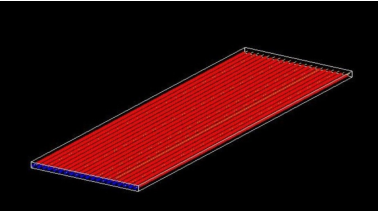
\includegraphics[width=0.6\textwidth]{STT_SimulationG4}
\end{cdrfigure}


\subsubsection{Design and prototyping of radiators and nuclear targets} 

As described in Section~\ref{cdrsec:detectors-nd-ref-fgt-stt}, a key
feature of the STT is the capability to integrate a series of
different nuclear targets for (anti)neutrino interactions.  The main
target is provided by the radiators made of thin polypropylene foils
(Figure~\ref{fig:STT_Detail}).  The design of the radiator targets has
been optimized with simulations of the Transition Radiation (TR) and
with emphasis on their integration into the mechanical structure of
the STT modules.  The production and design of the plastic foils was
discussed with vendors and we plan to produce a half-scale
(1.8~m$\times$1.8~m) prototype of the radiator targets to demonstrate
the assembly, the mechanical properties and the overall
performance. We have developed a preliminary design for the
pressurized Ar gas target (Figure~\ref{fig:STT_ArTargets}), based upon
the use of 0.5-in diameter aluminum tubes.  
\begin{cdrfigure}[Design of the target plane with pressurized Ar gas] 
{STT_ArTargets}{Design of the target plane with pressurized Ar gas.}
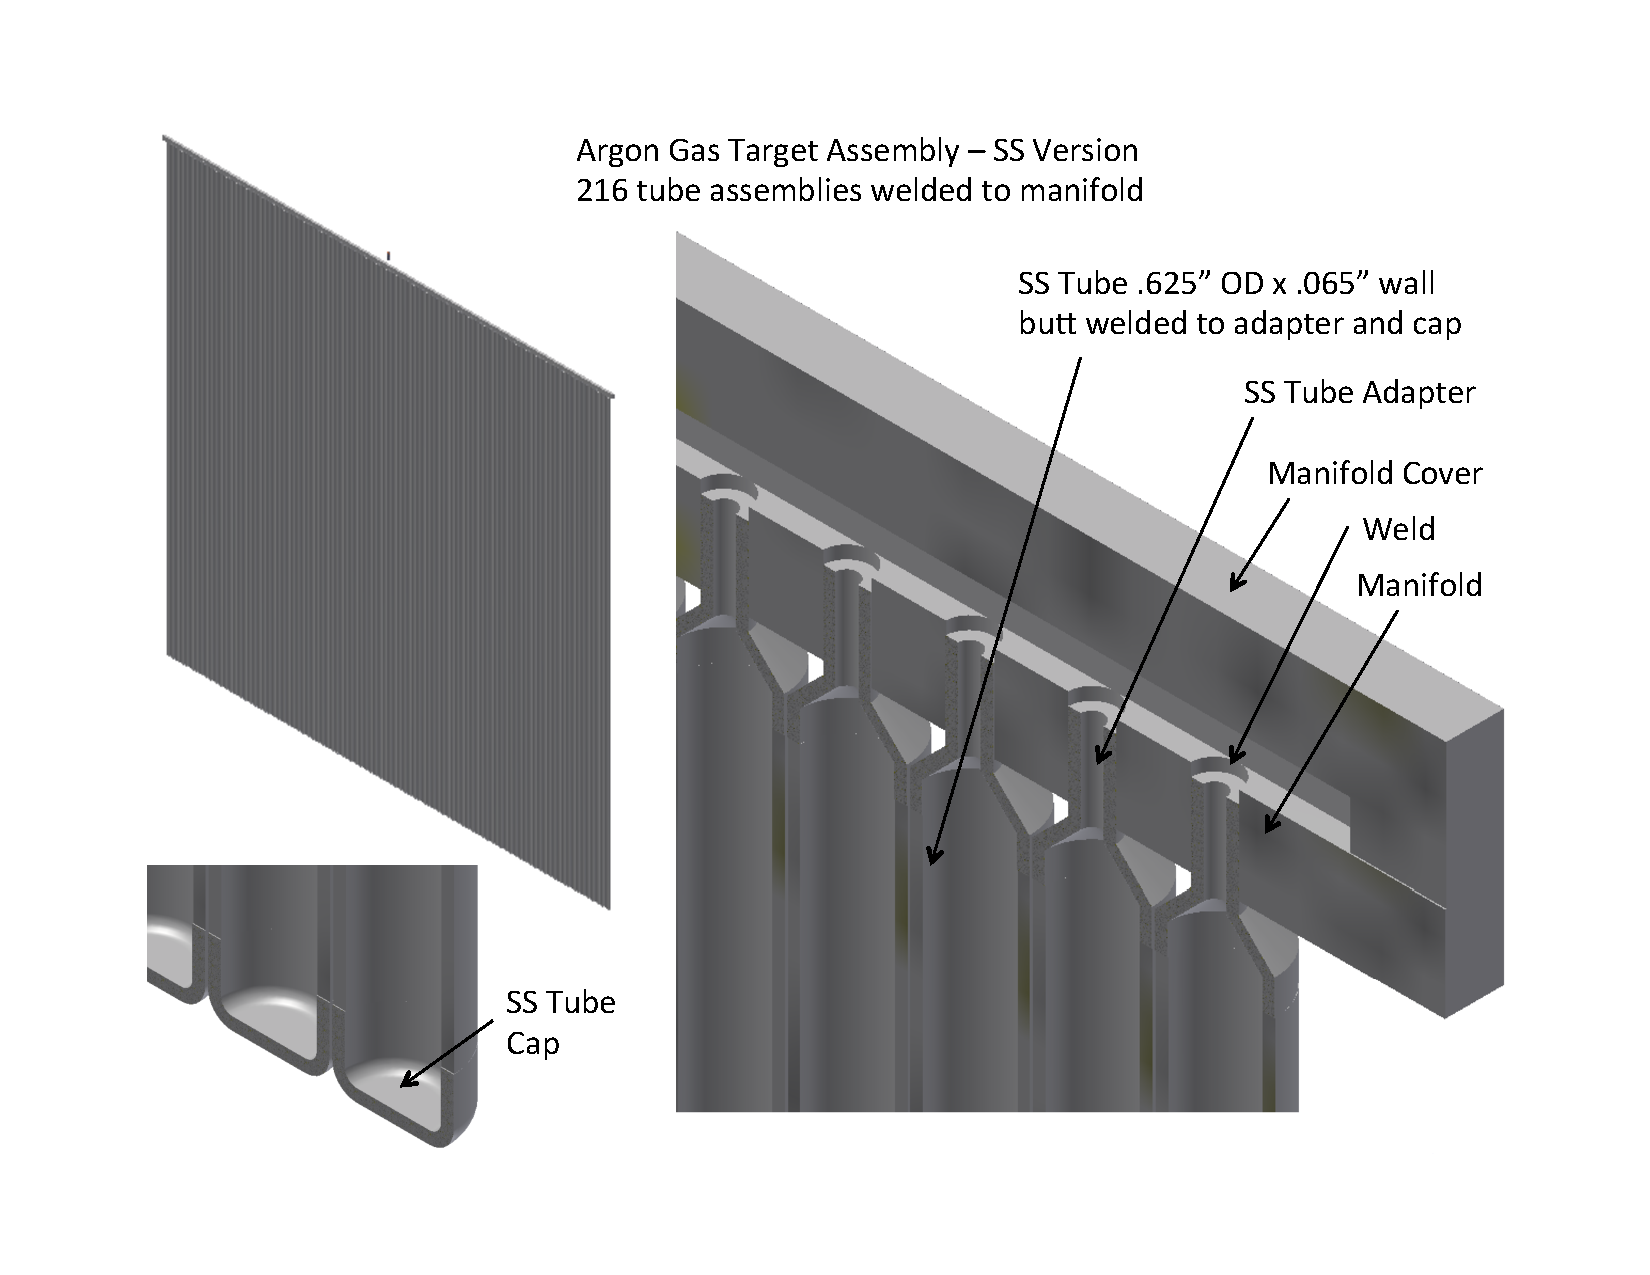
\includegraphics[width=0.6\textwidth]{STT_ArTargets}
\end{cdrfigure}
We plan to fabricate half-scale prototypes to test the concept and
further optimize the design of the tubes, including the tube diameter
and the possibility to use C-composite tubes.  Similarly, we plan to
build small-scale prototypes of the Ca and C targets.


\subsubsection{Anode Wire Studies} 

The sense wires used in the straw tubes were initially proposed to be
30~$\mu$m diameter Tungsten-Gold plated, similarly to the established
design of the COMPASS chambers. In order to minimize the material
budget of the mechanical frames used for the STT modules, it is
important to reduce the wire tension. To this end, the prototyping
includes a detailed study of the possibility to use 20~$\mu$m wires
instead of the default 30~$\mu$m. The tensile strength of these wires
inside the Straw Tubes could affect the signal generation over a long
period due to sagging so a detailed study is going on to study this
characteristic. Figure~\ref{fig:STT_WireTensionTests} shows the
tension measurements results for 20--30~$\mu$m wires using the induced
resonance method.  The proposed tension limit on the sense wires is
70~g.
\begin{cdrfigure}[Wire tension measurement studies (20~$\mu$m and 30~$\mu$m)]           
{STT_WireTensionTests}{Wire Tension Measurement studies for 20~$\mu$m and 30~$\mu$m.}
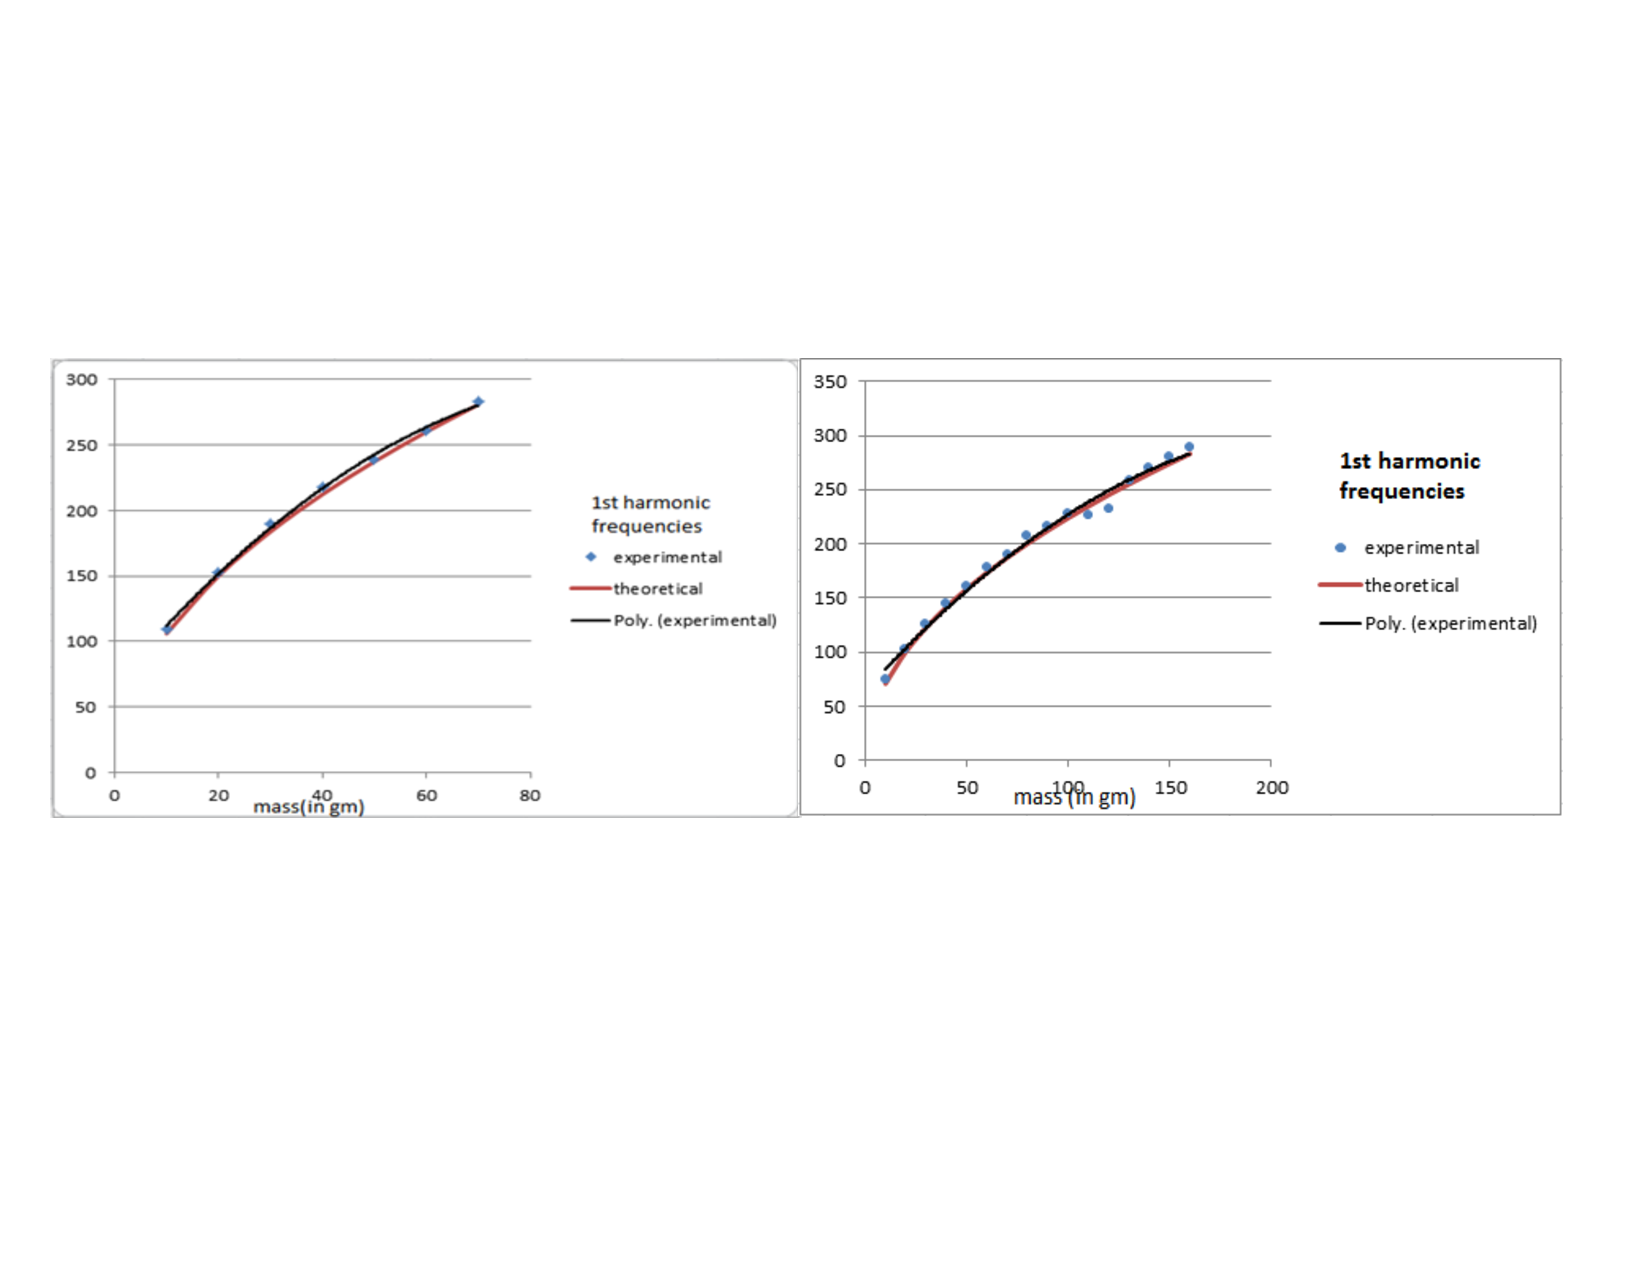
\includegraphics[width=1.0\textwidth]{STT_WireTensionTests}
\end{cdrfigure}


\subsubsection{Test Straw Chamber} 

A test chamber with 48 straws of the same dimensions as of FGT but
with 1~m length is available for operational studies to understand
the gas flow rates and for finalizing the pre-amplifier selection
parameters.  Figure~\ref{fig:STT_TestStrawChamber} shows the
operational pulse image with Ar+CO2 (80:20) gas taken with cosmic
rays. The voltage versus amplitude for one of the straws is also shown
in Figure~\ref{fig:STT_TestStrawChamber} to establish the QA/QC
procedure for the fabricated straws.
\begin{cdrfigure}[Pulse and voltage-amplitude for the test straw chamber]  
{STT_TestStrawChamber}{Example of pulse from the test straw chamber (left) and 
measurement of voltage vs. amplitude for one of the straws in the test chamber (right).}
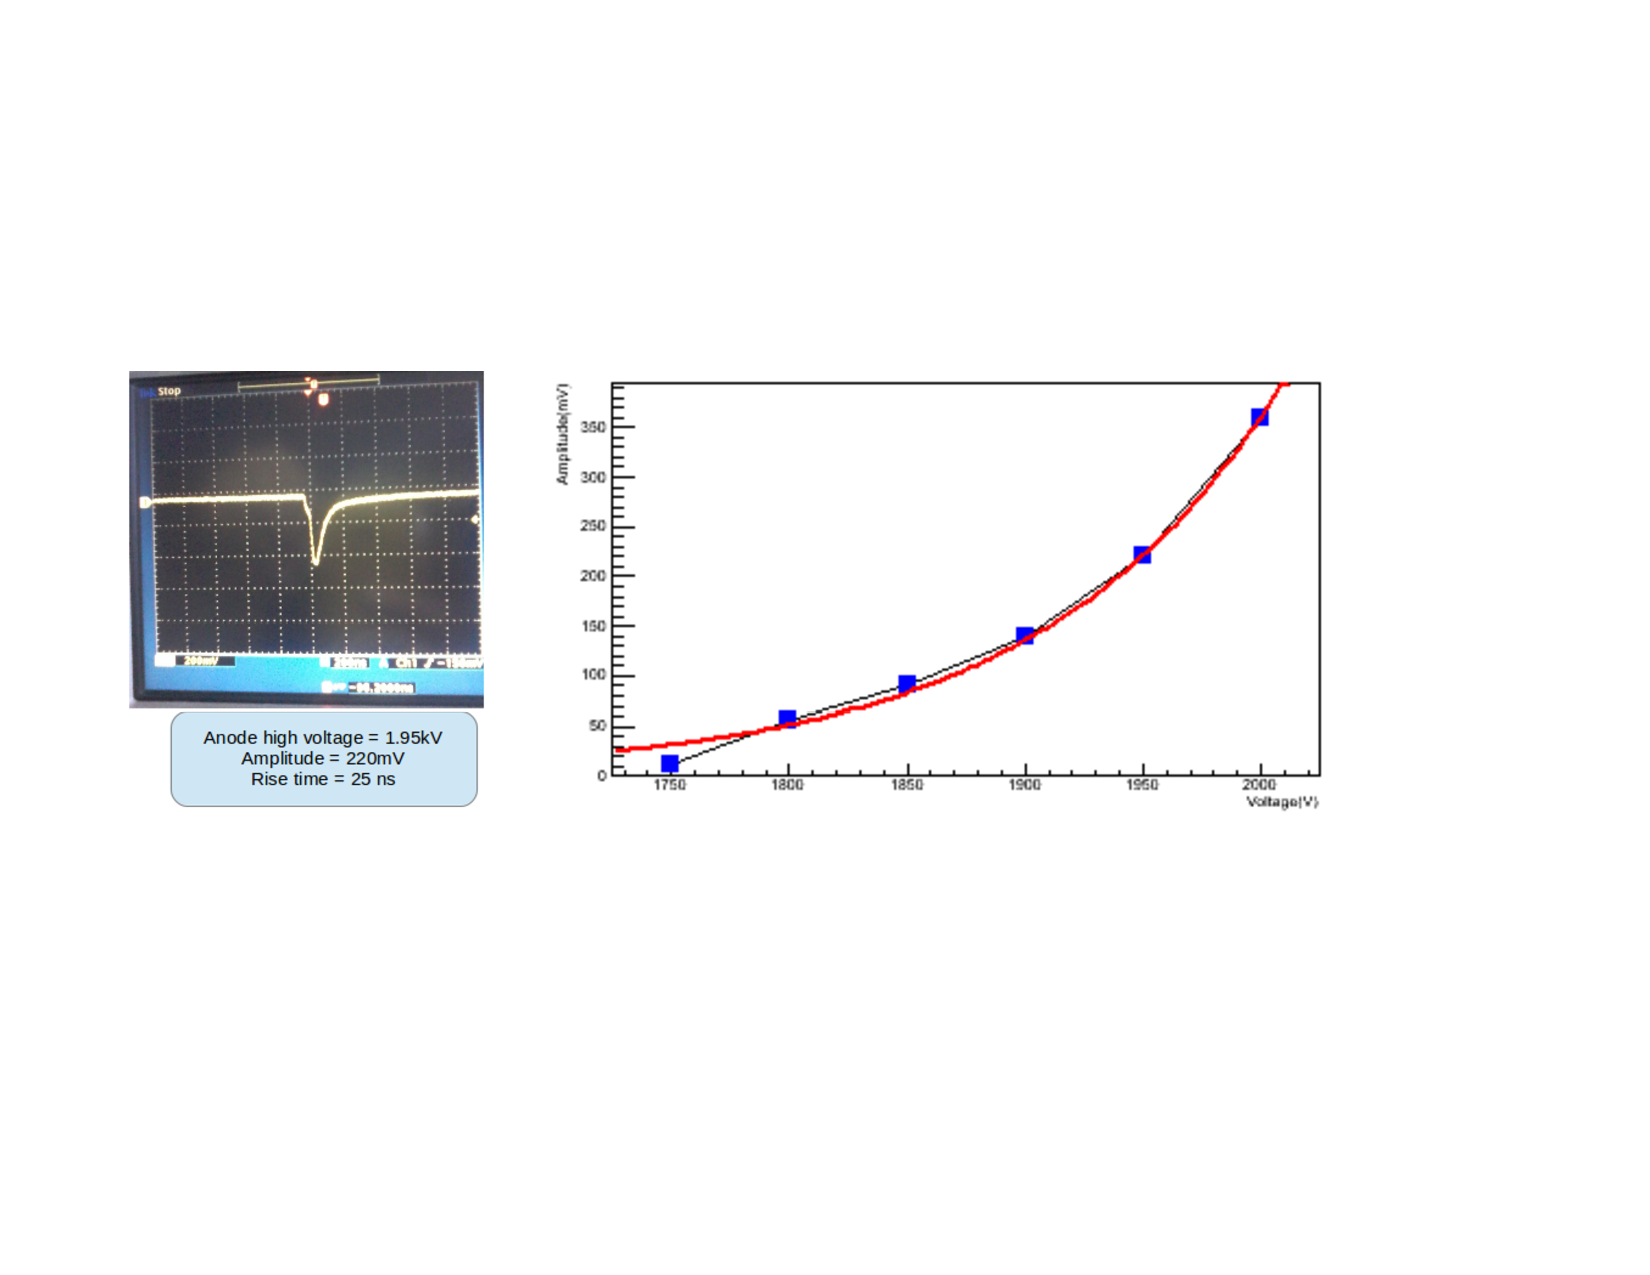
\includegraphics[width=1.0\textwidth]{STT_TestStrawChamber}
\end{cdrfigure}


\subsubsection{Front-end Electronics} 

Some tests are going on for the prototype stage electronics selection
for the signals to be read out.  A four channel pre-amplifier has been
tested with the test chamber using a radioactive source and the signal
has been recorded as shown in Figure~\ref{fig:STT_SignalPreAmp}.  The
backend DAQ is still worked out and would follow the description as
stated in Section~\ref{cdrsec:detectors-nd-ref-fgt-instrum}. At
present both CAMAC and VME based DAQ is available. $\mu$TCA based fast
DAQ has also been setup.
\begin{cdrfigure}[Signal from single straw using the BARC preamp and source]  
{STT_SignalPreAmp}{Signal from single straw using the BARC preamp and source.}  
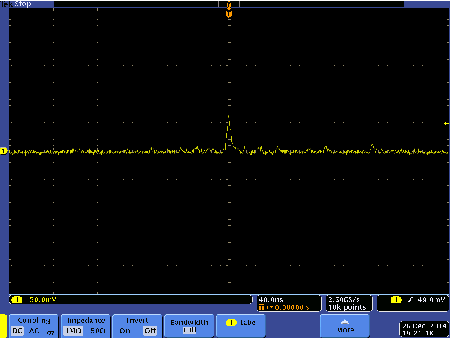
\includegraphics[width=0.6\textwidth]{STT_SignalPreAmp}
\end{cdrfigure}


\subsubsection{Other Activities}

As part of the prototyping, 50 Straws of 1.8~m from Lamina
Dielectrics Ltd., in UK, and 1~km of 30~$\mu$m anode wire from Luma
Sweden has been procured. The Optical bench for the fabrication of the
straws has been setup.  Two pre-mixed gas bottles of Ar+CO2 has been
procured. The operational gas mixture being Xe+CO2 will be added
soon. Local industry and vendors have been identified for the
manufacturing of nozzles, end-plugs, wire-spacers and steel
balls. Local workshops are available to fabricate the mechanical
structure to hold the straws in the prototype design and also to
fabricate a test stand for efficiency and characteristic studies with
a radioactive source. Wire stringing, straw gluing and other tooling
setups to be established.


\subsubsection{Design of the Full-scale STT Modules} 
 
We will optimize the final design of the STT modules based upon the
results obtained from the STT prototype and from the other prototyping
activities listed above. This task includes a detailed FEM analysis to
assess the mechanical structure and the choice of the final
materials. The final design is intended to be ready for the
fabrication of the full scale STT detector.



\subsection{ECAL Detector} 


The ECAL detector, as part of the FGT, will occupy the space outside
the STT with $4\pi$ coverage.  The detailed description of this
detector is given in Section~\ref{cdrsec:detectors-nd-ref-fgt-ecal}.
The ECAL prototype will be a 2~m$\times$2~m module similar to the
Downstream-ECAL design.  The half-scale downstream ECAL prototype
construction, which uses Pb as the absorber and extruded scintillator
with embedded fiber as the active detector system, will involve the
following steps:
\begin{itemize} 
\item Procure materials such as plastic scintillator bars, WLS fibers,
  SiPM, Pb sheets, etc.
\item Setup Mechanism to ensure the quality of the scintillator bars,
  fibers and Pb sheets.
\item Setup tools for the characterization of SiPM.
\item Assembly of scintillator bars in an Aluminum frame for a
  prototype layer formation
\item Undertake R\&D for the coupling of the fiber with SiPM as well
  as the inserting of fiber in the scintillator
\item Develop readout electronics for the prototype and setup a cosmic
  test stand with full DAQ
\item Mechanical stability of the ECAL design is being worked out
\end{itemize} 

The ECAL readout system is centered on a highly sensitive/high gain SiPM. The work to be undertaken 
during the R\&D phase will include:
\begin{itemize}
\item Comparison of SiPMs from Hamamatru, AdvanSiD and SiPM developed in India by SCL
\item Discussions are already on with all the vendors
\end{itemize} 

For optimizing the ECAL detector geometry, an effort for GEANT4
simulations of the ECAL has already been initiated. The geometry in
the current GEANT4 simulation includes 58 layers of alternating
horizontal and vertical scintillator layers per 1.75~mm Pb along the
z-direction. Each scintillator layer is made of plastic scintillator
bars of dimensions 4~m$\times$2.5~cm$\times$1~cm, resulting in 160
bars per layer and 9280 scintillator bars for the downstream ECAL in
the present configuration.  Figure~\ref{fig:ECAL_SimulationG4} shows
the longitudinal view of the electromagnetic shower in the downstream
ECAL by 2~GeV photons. Figure~\ref{fig:ECAL_detail} shows the design
of the Pb-scintillator assembly configuration for the ECAL.
\begin{cdrfigure}[Longitudinal view of EM shower in 
downstream ECAL by 2-GeV photons]  
{ECAL_SimulationG4}{Longitudinal view of the electromagnetic shower in 
the downstream ECAL by 2-GeV photons.}  
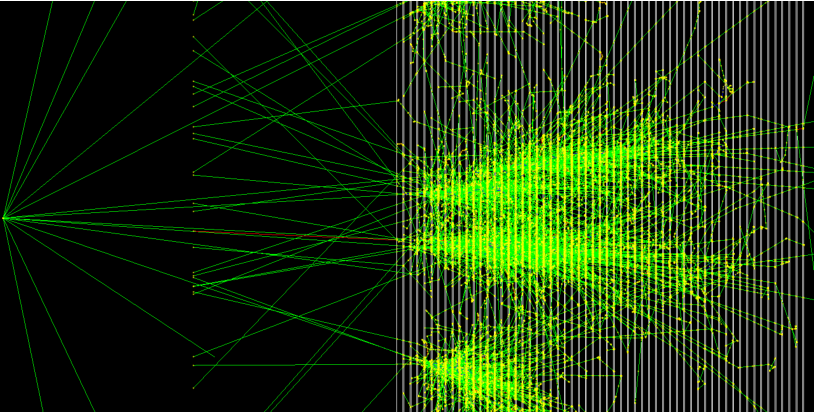
\includegraphics[width=0.6\textwidth]{ECAL_SimulationG4}
\end{cdrfigure}

For the construction of the prototype and final detector assembly a
space of dimension 32~m$\times$12~m has been
identified. Construction of a class 10,000 clean room covering a
laboratory space of 12~m$\times$12~m is under consideration
currently. Figure~\ref{fig:ECAL_LabIITG} shows the schematic diagram
of the laboratory refurbishment plan for the ECAL R\&D and fabrication
work.
\begin{cdrfigure}[Laboratory refurbishment plan for ECAL R\&D and assembly]  
{ECAL_LabIITG}{Laboratory refurbishment plan for the ECAL R\&D and assembly work.}  
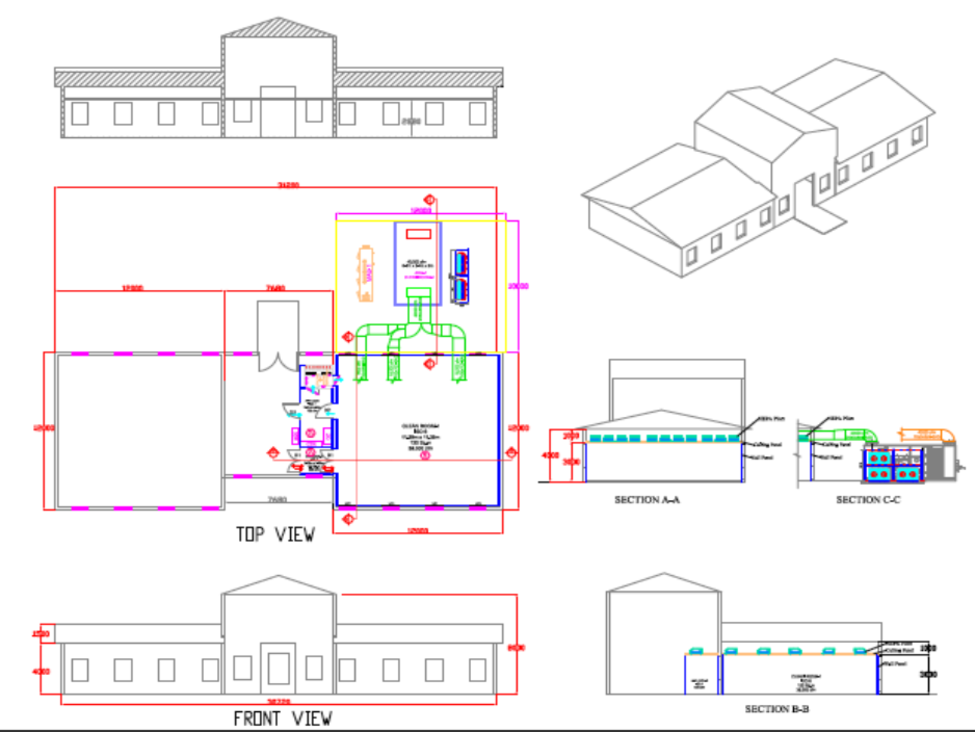
\includegraphics[width=0.6\textwidth]{ECAL_LabIITG}
\end{cdrfigure}


\subsection{Dipole Magnet Development} 

The massive dipole magnet (refer to
Section~\ref{cdrsec:detectors-nd-ref-fgt-magnet}) for the FGT will
play an exclusive role in the particle momentum measurements,
providing space for the MuID--RPCs installations in the magnet steel
and giving structural support to the FGT. The envisaged prototype of
the dipole magnet includes development of the tooling and
infrastructure to take up the engineering task.  The, thus developed,
infra-setup will be used to produce one C out of the total 8 Cs of the
8.0~m long dipole.  The same C will be utilized in the final magnet
assembly. In a similar way, one of the four coils would be assembled
too to establish the procedure of coil winding and measuring the
operating characteristics.  Field simulation work is already in very
advanced stage (see Figure~\ref{fig:Magnet_Bfield}) and the mechanical
designs (steel dimensions are being optimized to house the muon
identification detectors) are being produced.  Since it will be a
closed system, access to the inner detector systems is under extensive
study now.




\subsection{MuID--RPC Detector}   


Muons identification will done with the Resistive Plate Chamber
detectors made up of Bakelite electrodes.  The placeholders for these
RPCs will be provided by the magnet steel (on sides and ends). There
has been an extensive R\&D already done for such detectors. The
experience gained so far is being extended to the prototyping of the
muon identifiers. The dimensions of the electrodes make it a real
challenge to procure the raw material from industry. Now a local
industry has already been identified and a large 2.4~m$\times$1.2~m
RPC prototype has been assembled (see
Section~\ref{cdrsec:detectors-nd-ref-fgt-muonid}). The I-V
characteristics obtained for this RPCs are very encouraging. More such
RPCs will be fabricated during the prototyping phase and would be
tested for sustained efficiency over a period of time with variation
in ambient parameters as the Bakelite is sensitive to such
changes. Some of the measured quantities are shown in
Figure~\ref{fig:RPC_PrototypeTests}.  The readout electronics is being
developed by taking inputs from the similar R\&D done for the INO-ICAL
detector. The standard gases used in the RPC operations would need
substitutions/replacement with more safe gases and an initiative in
this direction will be taken up during the prototyping phase.
\begin{cdrfigure}[RPC characteristics measured during the prototype development]  
{RPC_PrototypeTests}{RPC characteristics measured during the prototype development.}  
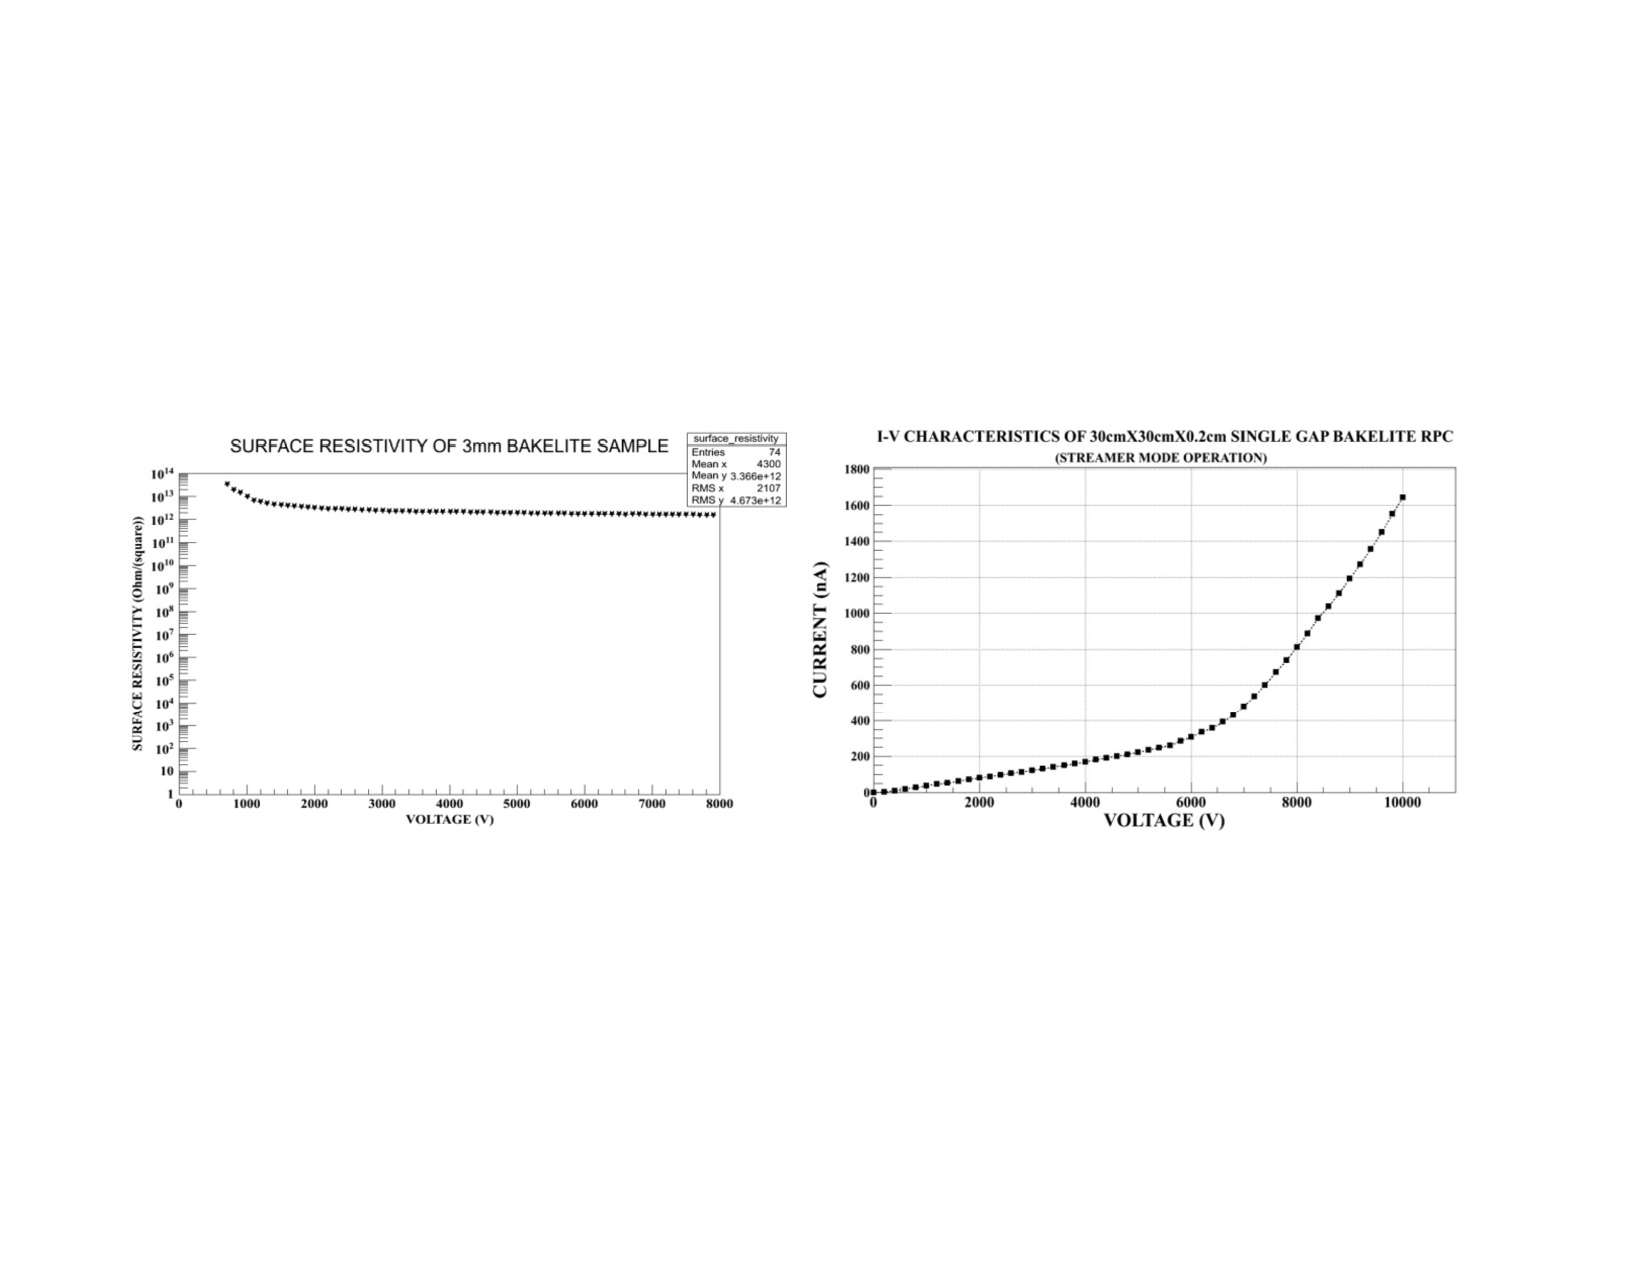
\includegraphics[width=1.0\textwidth]{RPC_PrototypeTests}
\end{cdrfigure}



\section{The ND Beamline Measurements Prototyping Plan} 
\label{sec:proto-nd-blm}

\subsection{Prototype Development for the Cherenkov and Ionization Detectors}
\label{subsec:proto-blm-muon-cherenkov-proto}

A prototype Cherenkov counter, along with associated fully automated
gas systems, HV systems, and data acquisition system has been
constructed and is undergoing testing in the NuMI neutrino beam's muon
alcove 2. In addition, three diamond detectors\cite{ref:CERNdiamond}
for ionization measurements have also been installed into the alcove.
Figure~\ref{fig:Alcove2Cherenkov} shows the prototype detectors in
NuMI alcove 2.
\begin{cdrfigure}[Muon gas Cherenkov counter]{Alcove2Cherenkov}
{A prototype muon gas Cherenkov detector for DUNE.  
Muons travel through an L-shaped 4" Conflat pipe filled with a 
pressurized gas. A flat mirror mirrors directs the optical photons 
to a photo multiplier. The lower right inset shows the 20~bar MKS 
pressure reading achieved by the Cherenkov gas system, and the inset 
on the upper right shows the CERN/Cividec diamond detectors mounted to the Cherenkov housing.}
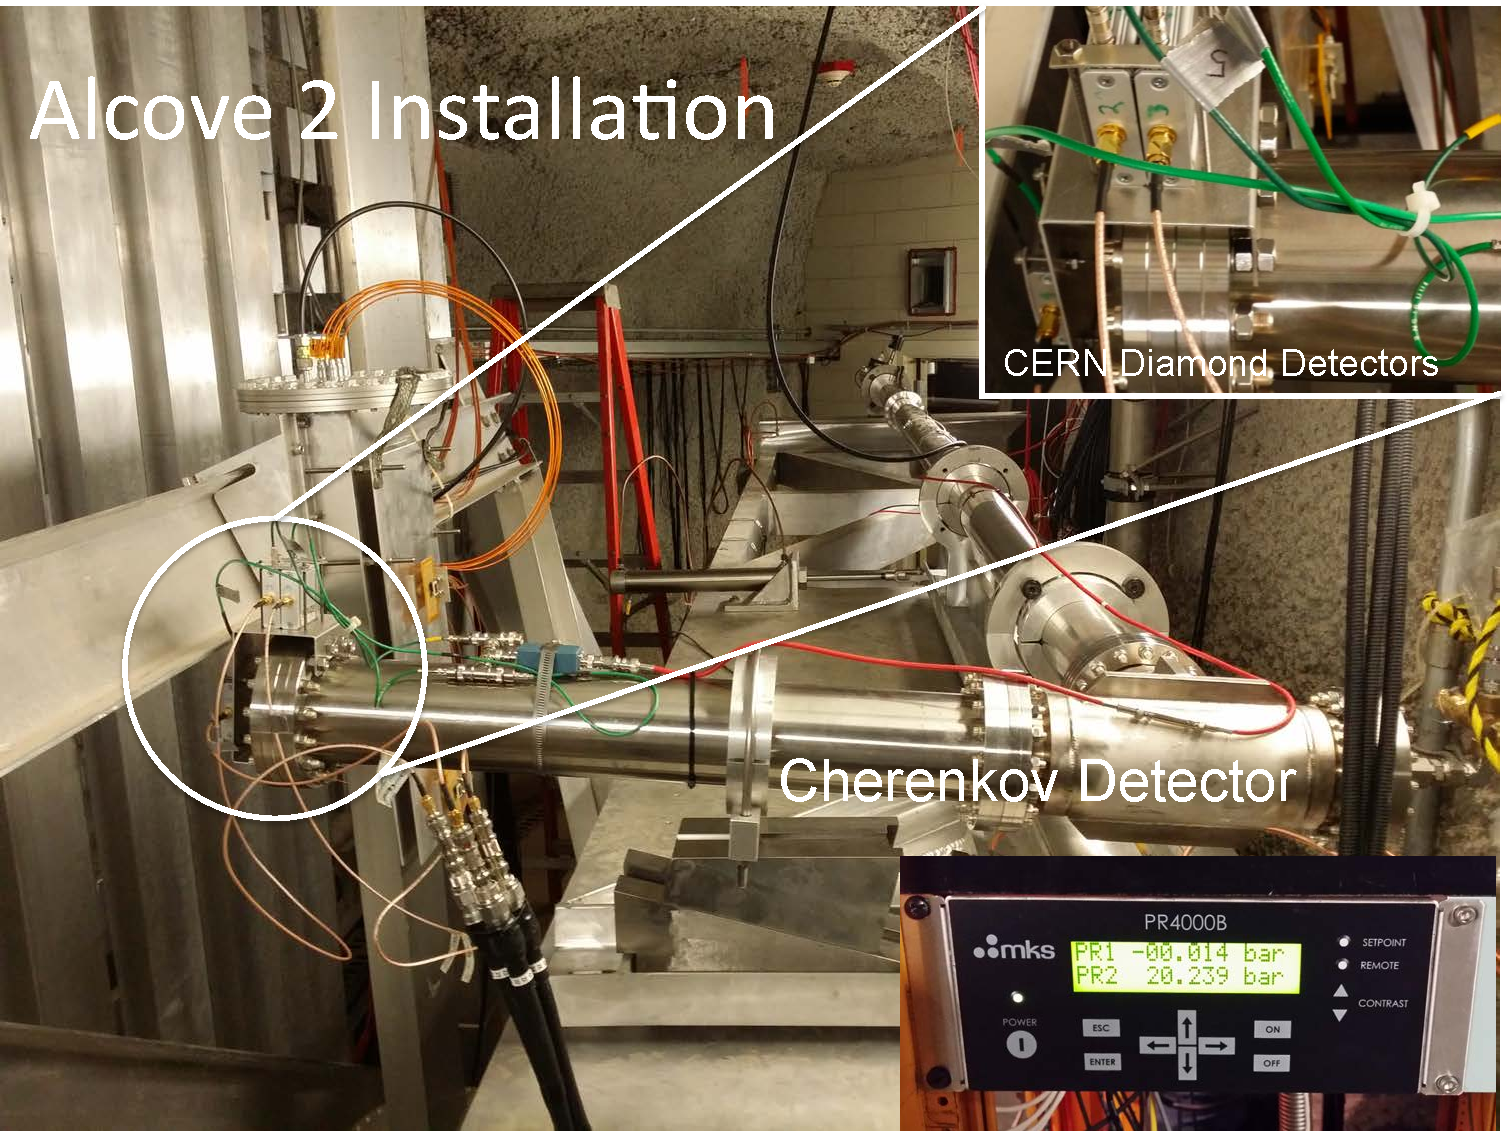
\includegraphics[width=6.in]{Alcove2Cherenkov}
\end{cdrfigure}

The counter has an automated gas system with a settable pressure that
ranges from vacuum to 20~atm, corresponding to muon Cherenkov
thresholds of 200~GeV/c and 1~GeV/c respectively. When operated at
vacuum, the PMT registers all background light unrelated to the gas,
e.g. transition radiation, light from particles hitting the window and
PMT glass.  Those contributions are observed to be very small relative
to the coherent, directional Cherenkov light.

The counter is constructed with a 1~m long radiator section as shown
in Figure~\ref{fig:CherenkovCounterDetail} . A 20~foot extension
allows the reflected Cherenkov light to travel to a sapphire pressure
window viewed by a photo multiplier tube.
\begin{cdrfigure}[Muon gas Cherenkov counter detail]{CherenkovCounterDetail}
{A prototype muon gas Cherenkov detector for DUNE.  }
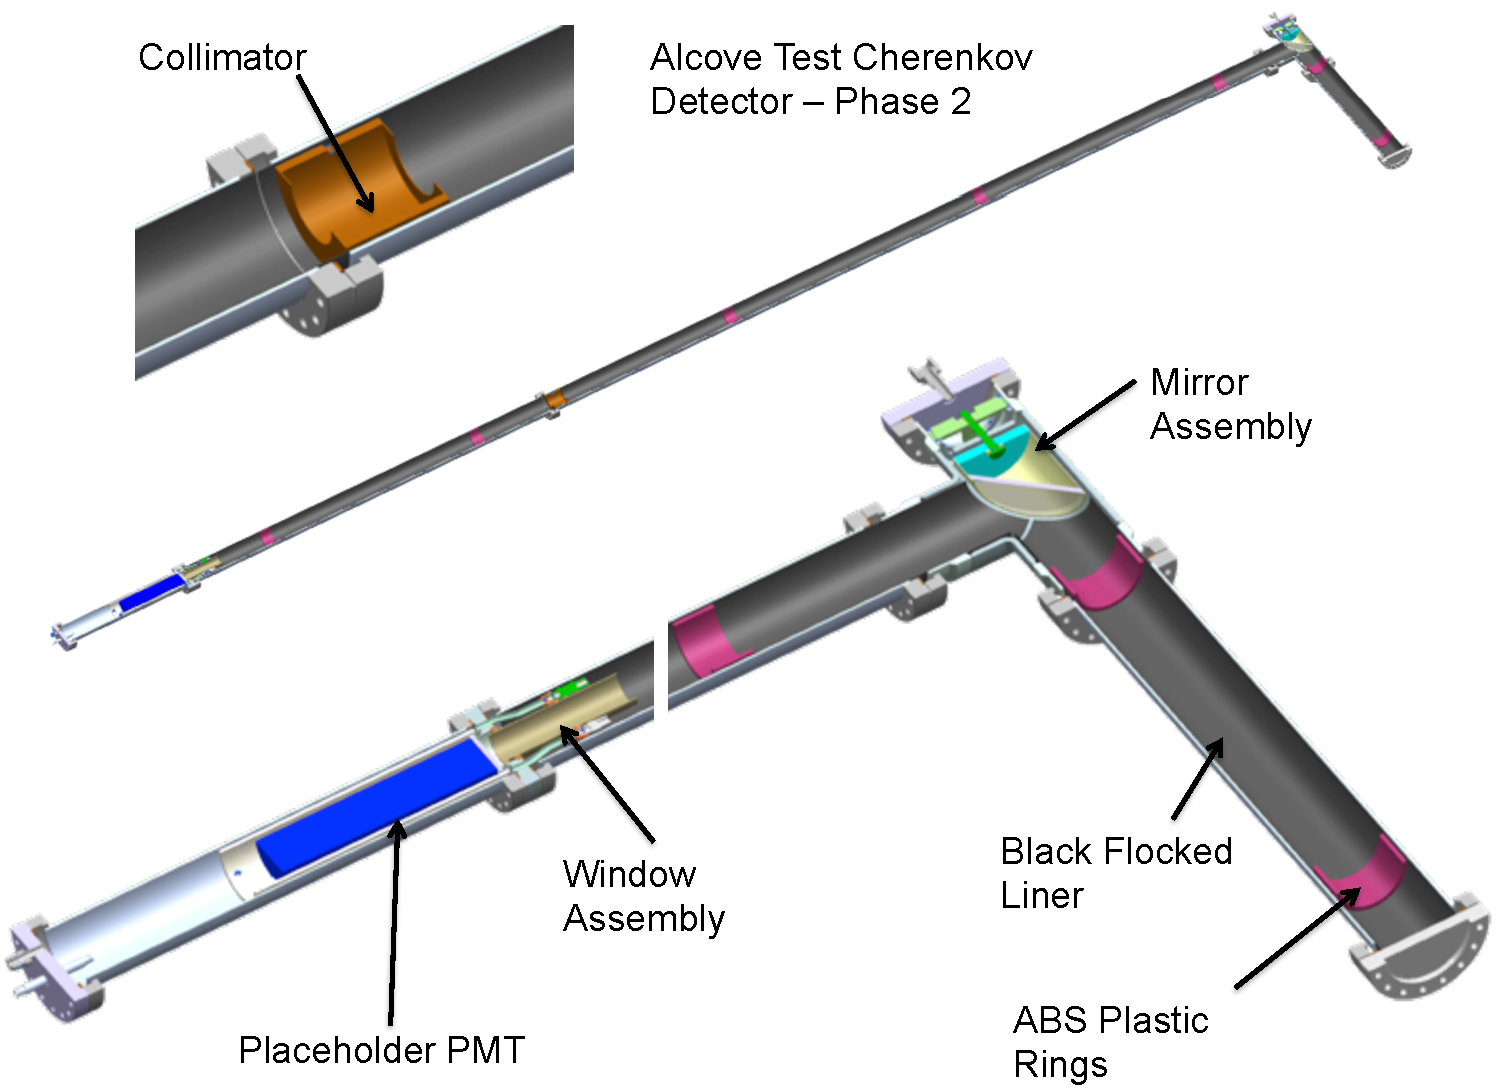
\includegraphics[width=6.in]{CherenkovCounterDetail.pdf}
\end{cdrfigure}


The prototype is now fully integrated into NuMI operations and
real-time waveforms can be viewed online as shown in
Figure~\ref{fig:MuonDetectorWaveforms}. 
\begin{cdrfigure}[Muon detector waveforms]{MuonDetectorWaveforms}
{The realtime display of the muon detector prototypes in operation 
on the NuMI beam line. The top two panels are the Cherenkov counter 
and CERN diamond detector\cite{ref:CERNdiamond}, The signals are 
transmitted through low-loss heliax cable, and then the waveform 
is digitized at 2.5~GHz with a 12~bit dynamic range, and the 
recorded onto disk storage for analysis. The signal from the 
muons is contained in the short beam pulse "buckets" created 
by the accelerator RF structure. The fast timing allows the 
prompt muon signal to be easily separated from potential backgrounds 
such as stopped muon decays, beta decays, and neutrons.}
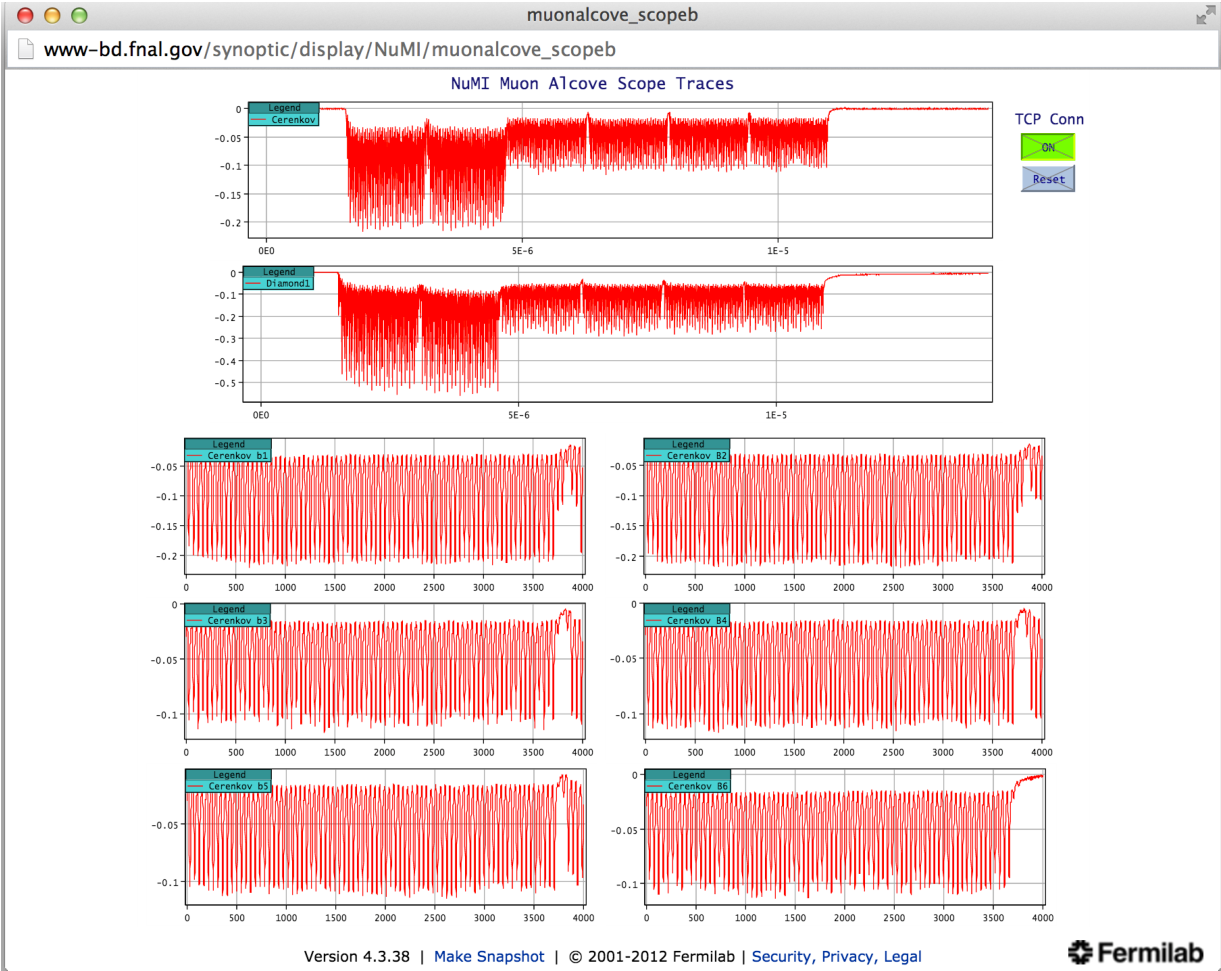
\includegraphics[width=5in]{MuonDetectorWaveforms}
\end{cdrfigure}
The top panel shows the waveform from the Cherenkov counter at 2~atm
gas pressure, that corresponds to a muon momentum threshold of
3~GeV/c. The second panel shows the waveform from a 9~mm$\times$9~mm
diamond detector mounted to the front flange of the Cherenkov radiator
section as shown in the inset of Figure~\ref{fig:Alcove2Cherenkov}.

The extracted NuMI proton beam, Resistive Wall Monitor (RWM) signal is
also recorded with an identical digitizer. That allows a direct,
bucket-by-bucket (individual proton pulses) comparison of the proton
current onto the NuMI primary proton target, and the muons measured
after the absorber with a 400~ps time resolution.



\subsubsection{Prototype Development of the Stopped Muon Counters}

Prototype development activity for the Michel-electron detectors will
be divided into studies of the rate and radiation environment where
the detectors will be located and development of the counters
themselves. 

The radiation environment will be studied both with Monte Carlo 
simulations and by measurements from initial prototype detectors 
in the NuMI muon alcoves\cite{ref:NuMIBeamMonitors}.
The prototypes will be installed into the alcoves in 2016 and 2017.
Studies will be performed to determine if the photon sensors
can survive the radiation environment at the location of the Michel
detector. If the sensors can survive, they can be attached directly to
the Cherenkov medium; if not, optical guides will have to bring the
light to a lower-radiation area to the side of the beam. Potential
radiation damage to the Cherenkov radiator itself will also be
studied.

The detector design will focus on selecting radiator and shielding
material, photon-detection technology and control/readout
hardware. Possible radiators include aerogel, which may be designed to
be replaced periodically, and flowing liquids such as H$_2$O or
mineral oil. Long-timescale saturation from the very high-rate
environment of the beam spill could affect the photon-counting
devices\cite{ref:HighRateCounting}. Thus, it will likely be necessary
to design fast-switching, high-voltage circuits that turn on the
photon counters in the first few microseconds after the spill is
over. A similar system was developed in the 1990s for the Brookhaven
Muon (g-2) Experiment~\cite{ref:G2} .

\subsection{Current Prototyping Activities}

A second set of muon detectors, the final DUNE design, are being
constructed at this time (2015). They are being installed directly
behind the NuMI proton beam dump (muon alcove 1). The detectors will
be mounted on a movable stand which has undergone an engineering
review at Fermilab. The entire setup, detectors and stand, will be
suitable for use in the DUNE beam.

The entire setup will be eventually transferred the DUNE absorber
hall. The higher radiation environment of alcove 1 will be more
similar to the eventual DUNE installation. It will allow the DUNE muon
detectors to be calibrated in the NuMI beam and ready for use in the
DUNE beam.
